\chapter{Computer Vision}

% ---------- Pixel Accuracy ----------
\clearpage
\thispagestyle{cvstyle}
\section{Pixel Accuracy}
\subsection{Pixel Accuracy}


Pixel Accuracy is one of the most straightforward evaluation metrics for image segmentation tasks. It measures the proportion
of correctly classified pixels across the entire image, comparing the predicted segmentation mask to the ground truth.

\noindent
\tikz{

\node[inner sep=2pt, font=\Large] (a) {
\centering
{
$\displaystyle
Pixel Accuracy = \frac{\sum_{j=1}^{k} {\color{nmlcyan}n_{jj}}}{\sum_{j=1}^{k} {\color{nmlpurple}t_{j}}}
$
}
};
\noindent
\draw[-latex,nmlcyan, semithick] ($(a.north)+(2.5,0.05)$) to[bend left=15] node[pos=1, right] {Correctly Predicted Pixels} +(1,.5); 
\draw[-latex,nmlpurple, semithick] ($(a.south)+(2.5,-0.05)$) to[bend left=15] node[pos=1, left] {Total Number of Pixels} +(-1,-.5); 
}
\vspace{-0.5\baselineskip} %

A Pixel Accuracy of 1.0 indicates perfect segmentation incase of balanced dataset, while lower values suggest a higher proportion of misclassified pixels.


\textbf{When to use Pixel Accuracy?}

Pixel Accuracy is useful when evaluating segmentation models where all pixel classes are of similar importance.
It provides a simple and interpretable measure of segmentation performance, making it a good starting point for initial
evaluation.

\coloredboxes{
\item Simple and interpretable.
\item Provides an initial sense of segmentation quality.
}
{
\item Insensitive to class imbalance. Heavily biased towards majority classes, leading to overly optimistic
evaluations in datasets with dominant background pixels.
\item Cannot differentiate per-class performance. A high Pixel Accuracy does not guarantee that all classes are well-segmented.
}

\clearpage

In the example below, there are three classes: 0, 1, and 2. The ground truth contains all three classes, but the model’s predictions do not contain a single instance of class 2. 


\newcolumntype{C}[1]{>{\centering\arraybackslash}m{#1}}

\renewcommand{\arraystretch}{1.5}



 \begin{minipage}{0.5\linewidth}
    \setcounter{table}{0}
  \centering
  \begin{tabular}{|C{1.5cm}|C{1.5cm}|C{1.5cm}|}
\hline
\cellcolor[HTML]{d8beff} 0 & \cellcolor[HTML]{d8beff} 0 & \cellcolor[HTML]{ffde59} 1 \\
\hline
\cellcolor[HTML]{d8beff} 0 & \cellcolor[HTML]{ffde59} 1 & \cellcolor[HTML]{ffde59} 1 \\
\hline
\cellcolor[HTML]{ffde59} 1 & \cellcolor[HTML]{95e8ed}  2 & \cellcolor[HTML]{95e8ed} 2 \\
\hline
\end{tabular}
 \end{minipage}%
%
 \begin{minipage}{0.5\linewidth}
    \setcounter{table}{0}
  \centering
  \begin{tabular}{|C{1.5cm}|C{1.5cm}|C{1.5cm}|}
\hline
\cellcolor[HTML]{d8beff} 0 & \cellcolor[HTML]{d8beff} 0 & \cellcolor[HTML]{ffde59} 1 \\
\hline
\cellcolor[HTML]{d8beff} 0 & \cellcolor[HTML]{ffde59} 1 & \cellcolor[HTML]{d8beff} 0 \\
\hline
\cellcolor[HTML]{ffde59} 1 &  \cellcolor[HTML]{ffde59} 1 & \cellcolor[HTML]{ffde59} 1 \\
\hline
\end{tabular}
 \end{minipage}%


Despite this,

\[
\text{Pixel Accuracy} = \frac{\text{Correctly predicted pixels}}{\text{Total number of pixels}} = \frac{6}{9} \approx 66\%
\]

Pixel accuracy therefore reflects overall correctness but does not reveal whether the model performs poorly on minority classes. 
This is to show that high PA does not necessarily indicate superior segmentation performance.

To compensate for this, Mean Pixel Accuracy (MPA), calculates accuracy per class and then averages across all classes.
This adjustment ensures that smaller classes are not overshadowed by dominant ones, making MPA a more balanced evaluation
metric in class-imbalanced datasets.

\orangebox{Did you know that...}
{Pixel Accuracy is part of a family of semantic segmentation evaluation metrics. 
This family includes several related measures that each capture different aspects of performance.
They can be sub-grouped into pixel level metrics, region/overlap based metrics, and class balanced metrics.}

\textbf{Other related metrics}
Other metrics in this family are Mean Pixel Accuracy (mPA), Intersection over Union (IoU) and Frequency Weighted IoU (FWIoU).



% ---------- PCK ----------
\clearpage
\thispagestyle{cvstyle}
\section{Percentage of Correct Keypoints}
\subsection{PCK}

A keypoint is a specific landmark on an object like an elbow, knee, or ankle in human pose estimation.

PCK measures the percentage of predicted keypoints that are close enough to their true positions.

\begin{center}
\tikz{
    \node[inner sep=2pt, font=\Large] (a) {
        $\displaystyle
        PCK(\alpha) = \frac{1}{\textcolor{nmlgreen}{N}} \sum_{i=1}^{N} 1\!\left(\textcolor{nmlpurple}{d_i} \le \textcolor{nmlyellow}{\alpha L}\right)
        $
    };
    \draw[-latex,nmlyellow, semithick] ($(a.north)+(0.5,0.05)$) to[bend left=15] 
        node[pos=1, right] {Threshold Radius} +(1,.5); 
    \draw[-latex,nmlgreen, semithick] ($(a.south)+(-1.15,-0.1)$) to[bend left=15] 
        node[pos=1, left] {Number of Keypoints} +(-1,-.5); 
    \draw[-latex,nmlpurple, semithick] ($(a.south)+(1.2,0.05)$) to[bend right=15] 
        node[pos=1, right] {Euclidean Distance} +(1,-.5); 
}
\end{center}

For each keypoint $i$, we measure the Euclidean distance $d_i$ between the prediction and the ground truth.
A prediction is considered correct if $d_i$ is less than or equal to the threshold radius $\alpha L$, where $L$ is a reference length (for example, head size or torso length).


\textbf{When to use PCK?}

PCK is suited for tasks where you care about relative keypoint accuracy rather than raw pixel error.
It works well in applications like human pose estimation, facial landmark detection, or object keypoint detection. 

\coloredboxes{
\item Scale Invariance. By normalizing the threshold based on body part size or image scale, PCK accounts for different
object sizes.
\item Robust to minor localization errors. Small deviations from the exact keypoint location do not significantly impact
the score.
}
{
\item The performance can vary significantly depending on the chosen threshold $\tau$, making comparisons difficult across
studies.
\item Not Differentiable. Since it is a threshold-based metric, it cannot be directly used as a loss function for training
deep learning models.
}
\clearpage

\begin{figure}[htbp]
    \centering
    \hspace*{-0.5cm}
    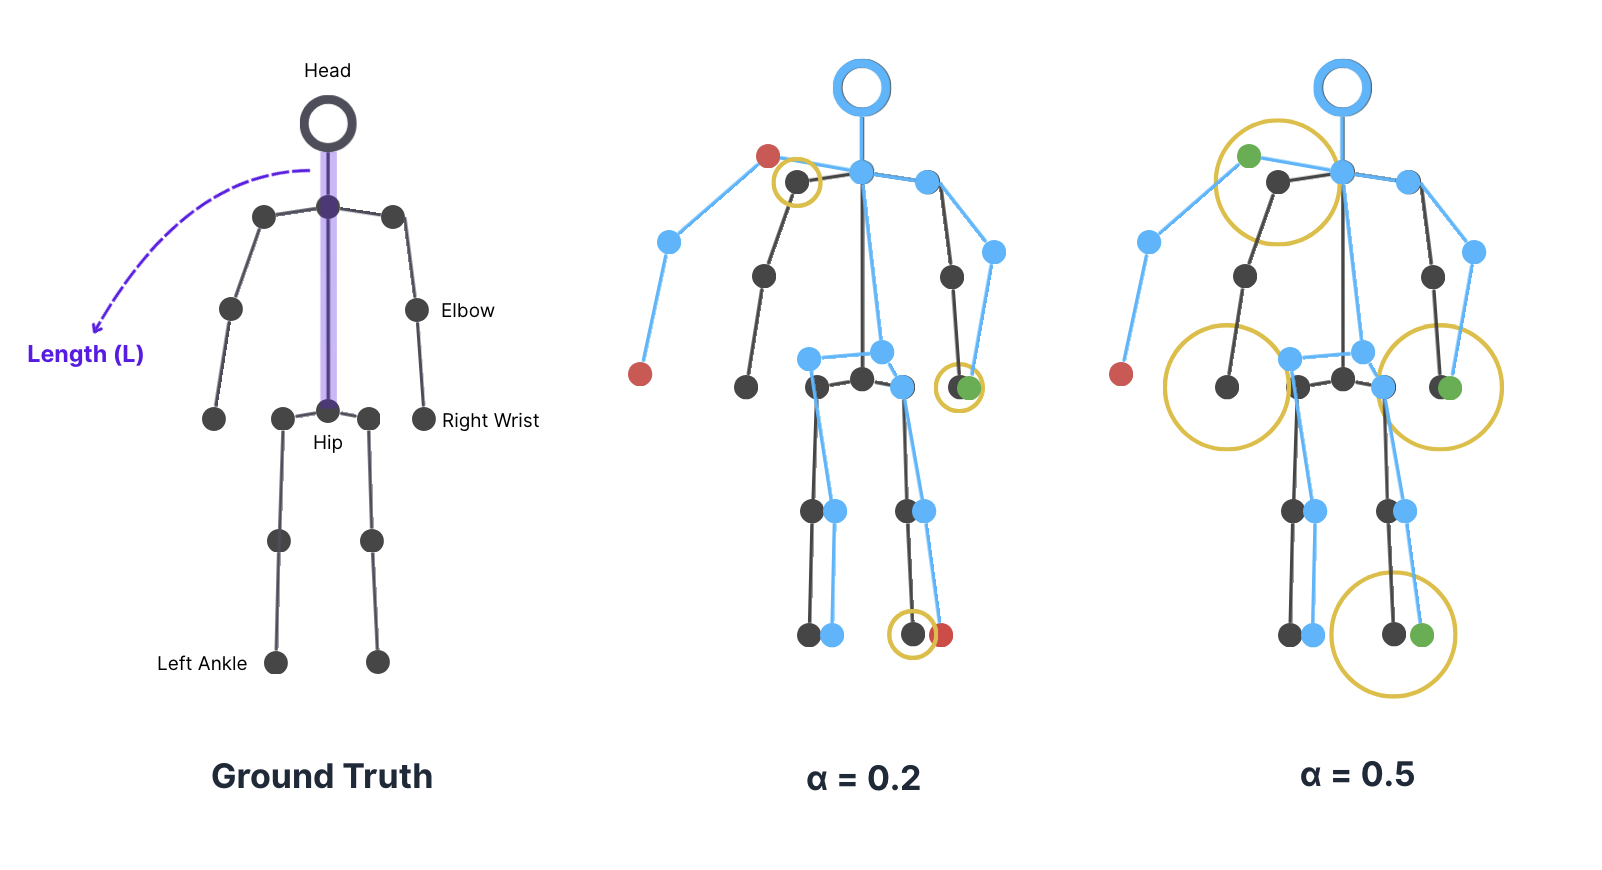
\includegraphics[width=1.1\textwidth]{figures/PCK_threshold_visual.png} % Full width
    %\caption{Only the predictions within the threshold radius is considered correct.}
    \label{fig:PCK_threshold}
\end{figure}

To find correct keypoint(green), we determine whether the predicted keypoint (blue) falls within a threshold distance from the ground truth (black).  
The threshold is defined as a fraction $\alpha$ of a reference length $L$, typically the torso length.  

The radius of the circle around each ground-truth joint is $r = \alpha \cdot L$.  

In practice, we choose a small $\alpha$ for high-precision tasks, such as hand or facial keypoint detection.  
We use a larger $\alpha$ when approximate locations suffice, for example in full-body pose estimation for activity recognition.


\orangebox{Did you know that...}
{A popular variant, \textbf{PCKh}, uses head size as the reference length \(L\). }

% ---------- OKS ----------
\clearpage
\thispagestyle{cvstyle}
\section{Object Keypoint Similarity}
\subsection{OKS}

Object Keypoint Similarity (OKS) generalizes PCK by replacing the hard threshold with a continuous similarity score.  

Where PCK counts a keypoint as correct if it falls within a circle of radius $\alpha L$, OKS assigns a value between 0 and 1 based on how far the predicted keypoint is from the ground truth, normalized by object scale and keypoint-specific tolerance.

\noindent
\tikz{
\node[inner sep=2pt, font=\Large] (a) {
\centering
{
$\displaystyle
{similarity}_i = \exp\!
  -\,\frac{{{distance error}}^{2}}{ {{object scale}}^{2} \, {{tolerance}_i}^{2} }
$
}
};
}

\textbf{When to use OCK?}

OKS is particularly suited for evaluating pose estimation and keypoint-based object detection models, such as: human pose
estimation, facial landmark detection and benchmarking keypoint models.


\coloredboxes{
\item Scale-invariant evaluation. Unlike raw pixel-based metrics, OKS normalizes errors relative to object size,
ensuring fair evaluation across small and large objects.
\item Smooth penalization of localization errors.
Instead of a hard threshold (like in PCK), OKS applies a Gaussian function to penalize errors, making it a more continuous
and informative measure.
\item Handles occlusions and visibility issues. The visibility flag $v_i$ ensures that models are not penalized for missing
occluded or unlabeled keypoints.
}
{
\item Requires keypoint-specific constants. The $k_i$ values must be tuned per dataset, making cross-dataset comparisons
challenging.
\item Computationally more complex than PCK.
}

\clearpage
\orangebox{Did you know that...}
{OKS is the standard metric for evaluating pose estimation models in the COCO Keypoint Challenge, influencing the development
of state-of-the-art architectures like OpenPose, HRNet, and DEKR.}


% ---------- PSNR ----------
\clearpage
\thispagestyle{cvstyle}
\section{PSNR}
\subsection{Peak Signal-to-Noise Ratio}

In image generation and reconstruction, it is important to measure how closely the generated images resemble reference images.
PSNR is a widely used metric that quantifies pixel-level differences.

% equation
\begin{center}
    \tikz{
        \node[inner sep=2pt, font=\Large] (a) {
            {
                $\displaystyle
                    PSNR = 10 \cdot \log_{10}\left(\frac{\color{nmlred}MAX^2}{\color{nmlpurple}MSE}\right)
                $
            }
        };
        \draw[-latex,nmlred, semithick] ($(a.north)+(2.1,-0)$) to[bend right=15] node[pos=1, left] {maximum possible pixel}
        +(-1,.5); 
        \draw[-latex,nmlpurple, semithick] ($(a.south)+(2,-0.1)$) to[bend left=15] node[pos=1, left] {mean squared error}
        +(-1,-.5);
    }
\end{center}

\vspace{-10pt} 

where given an original image $O$ of size $h \times w$ and a reconstructed image $R$, the $MSE$ is defined as:

\vspace{-10pt}

% equation
\begin{center}
    \tikz{
        \node[inner sep=2pt, font=\large] (a) {
            {
                $\displaystyle
                 MSE = \frac{1}{\color{teal!70!green}h \cdot \color{nmlcyan}w} \sum_{i=1}^{h} \sum_{j=1}^{w}
                 \left(\color{nmlred} O(i,j) \color{black} - \color{nmlpurple} R(i,j) \right)^2
                $
            }
        };
        \draw[-latex,teal!70!green, semithick] ($(a.west)+(1.7,-0.5)$) to[bend left=15] node[pos=1, left] {height} +(-1,-.5); 
        \draw[-latex,nmlcyan, semithick] ($(a.west)+(2.4,-0.5)$) to[bend right=15] node[pos=1.62, left] {width} +(1,-.5);
        \draw[-latex,nmlred, semithick] ($(a.south)+(1,0.5)$) to[bend right=15] node[pos=1, right] {original pixel value}
        +(1,-.5);
        \draw[-latex,nmlpurple, semithick] ($(a.north)+(2.3,-0.4)$) to[bend right=15] node[pos=1, left] {reconstructed pixel
        value} +(-1,.5);    
    }
\end{center}

\vspace{-10pt}

The intuition behind PSNR is that it expresses how large the possible signal value is in comparison to the error. 
If the error is subtle compared to the maximum signal (i.e., a high PSNR), the reconstructed image is relatively similar to
the target in terms of pixel values. The unit of peak signal-to-noise ratio is decibel (dB) and the image have PSNR from 30 dB
could be consider as good reconstruction quality.



\textbf{When to use PSNR?}

PSNR is often chosen as the first metric to provide an overview of how closely the generated image matches the target.

\coloredboxes{
\item It is a straightforward and widely accepted standard for comparing vision algorithms.
\item Simple and fast to compute.
}
{
\item It is not always align with human perception of image.
\item PSNR is sensitive to even small global changes in lighting, contrast, or color.
}

\clearpage

\thispagestyle{customstyle}


\begin{figure*}[ht!]
    \centering
    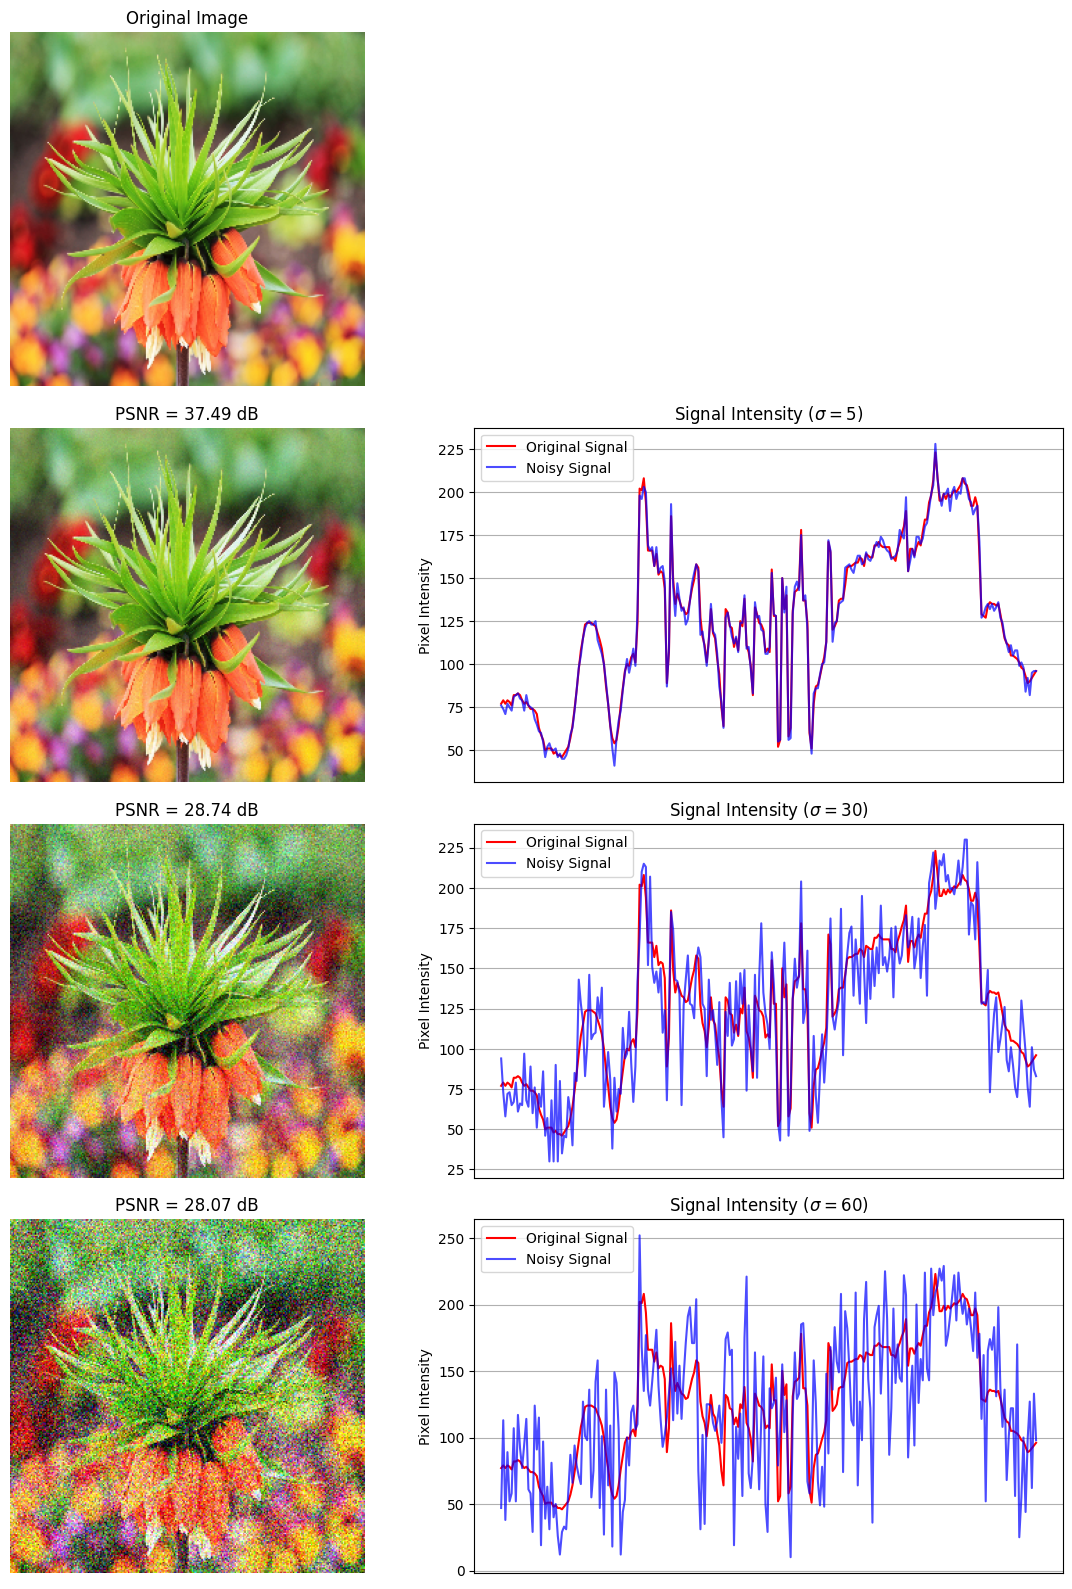
\includegraphics[width=0.6\textwidth]{figures/PSNR_plot.png}
    % \caption{Caption}
    \label{PSNR plot}
\end{figure*}


\textbf{Figure 7.1 Image with different PSNR.} Demonstrates noisy images with their corresponding PSNR values compared to the
original ones. \textbf{Left:} Original image and its noisy version. 
\textbf{Right:} Illustration of how strong noise signals have been added to the original image.
The color image is from the popular \href{https://data.vision.ee.ethz.ch/cvl/DIV2K/}{DIV2K} dataset.
\vspace{-12pt} 

\orangebox{Did you know that...}
{PSNR is not just for images; it can be applied to \textbf{video, audio, or even signal processing}. Anytime we want to
measure the quality of \textbf{reconstructed} signal compared to the \textbf{original}, PSNR could be considered.}

\vspace{-5pt} 

\textbf{Other related metrics}

\vspace{-5pt} 

Modern computer vision problems often focus on generating likely realistic images that are perceptually pleasing to humans,
rather than strictly matching the
target image pixel by pixel. Therefore, PSNR is typically used in conjunction with other modern metrics like Fréchet Inception
Distance (FID) or Inception Score (IS).


% ---------- Sørensen–Dice Coefficient ----------
% references: 
% https://rosettacode.org/wiki/Sorensen%E2%80%93Dice_coefficient
% https://distancia.readthedocs.io/en/latest/SorensenDice.html
\clearpage
\thispagestyle{cvstyle}
\section{S{\o}rensen–Dice Coefficient}
\subsection{S{\o}rensen–Dice Coefficient}


The S{\o}rensen–Dice Coefficient, sometimes simply called the Dice score, is a similarity metric that
measures the overlap between two sets. In computer vision, it is often used to evaluate segmentation
models by comparing the predicted mask against the ground-truth mask.

% equation
\begin{center}
    FORMULA GOES HERE
\end{center}

where $A$ is the set of predicted positives and $B$ is the set of true positives.
The score ranges between 0 and 1, with 1 indicating perfect overlap and 0 indicating no overlap.
When applied to binary classification problems, the S{\o}rensen–Dice coefficient is mathematically
equivalent to the F1-score.

\textbf{When to use S{\o}rensen–Dice Coefficient?}

Use the S{\o}rensen–Dice Coefficient when you need a robust measure of similarity between two binary
or categorical sets. It is especially popular in immage segmentation, information retrieval and
natural language processing.

\coloredboxes{
\item Intuitive and interpretable. Directly measures the overlap between predicted and true sets.
\item Balances false positives and false negatives. Equivalent to F1-score, making it well-suited to
imbalanced data.
}
{
\item Not a true metric, as it does not satisfy the triangle inequality.
\item Overly optimistic in some contexts. May give high similarity even when boundary alignment
is poor, which matters in precise applications like medical imaging.
}

\clearpage

\thispagestyle{customstyle}

\orangebox{Did you know that...}
{The S{\o}rensen–Dice coefficient was first introduced in ecology as a way to measure the similarity
between populations of flora and fauna.}

\vspace{-5pt}


% ---------- Panoptic Quality ----------
% references: 
% https://openaccess.thecvf.com/content_CVPR_2019/papers/Kirillov_Panoptic_Segmentation_CVPR_2019_paper.pdf
% https://www.nature.com/articles/s41598-023-35605-7
\clearpage
\thispagestyle{cvstyle}
\section{PQ}
\subsection{Panoptic Quality}

Panoptic Quality (PQ) is a computer vision metric designed to evaluate panoptic segmentation, a task
that unifies semantic segmentation and instance segmentation . Unlike earlier metrics that treated stuff
(amorphous regions like sky, road) and things (countable objects like cars, people) separately,
PQ evaluates both in a uniform and consistent way.

% equation
\begin{center}
    FORMULA GOES HERE
\end{center}

PQ can be decomposed into two interpretable components:
% equation
% Segmentation Quality (SQ): the average IoU of matched segments.
% Recognition Quality (RQ): an F1-like measure that penalizes false positives and false negatives.

\begin{center}
    $PQ = SQ \times RQ$
\end{center}

\textbf{When to use Panoptic Quality?}

Use PQ when evaluating models that must both classify and segment objects at the pixel level, such
as in autonomous driving, medical imaging, or robotics. It is especially relevant when your model
must handle both “stuff” classes and “thing” classes.


\coloredboxes{
\item Unified evaluation: Handles both stuff and things in a single metric.
\item Balanced penalties. The denominator includes $FP$ and $FN$, ensuring both missed and spurious
predictions are penalized.
\item Interpretability: The $SQ$ and $RQ$ decomposition makes it easy to diagnose whether errors
come from poor segmentation or recognition.
}
{
\item Equal weighting of segments. While useful for fairness, this may undervalue large, important regions in favor of many small segments.
\item Boundary insensitivity: Since PQ relies on IoU, it may miss fine-grained boundary quality,
which can matter in domains like medical imaging.
}

\clearpage

\thispagestyle{customstyle}

\orangebox{Did you know that...}
{Panoptic Quality was designed not only as a metric but also as a driver for task definition. The authors
hoped that having a unified metric would accelerate the adoption of panoptic segmentation as a new standard
task in vision research.}


% ---------- Structural Similarity Index ----------
% references: 
% https://www.cns.nyu.edu/pub/lcv/wang03-preprint.pdf
% https://scikit-image.org/docs/0.25.x/auto_examples/transform/plot_ssim.html (has a good visual)
% https://espace2.etsmtl.ca/id/eprint/12070/1/Noumeir%20R.%202015%2012070%20Limitations%20of%20the%20SSIM%20quality%20metric.pdf?utm_source=chatgpt.com

\clearpage
\thispagestyle{cvstyle}
\section{SSMI}
\subsection{Structural Similarity Index}

The Structural Similarity Index Measure (SSIM) is a computer vision metric that evaluates the similarity
between two images by modeling perceived changes in structural information, rather than relying solely on
pixel-level differences. Unlike metrics such as MSE or PSNR, which compare absolute differences, SSIM
incorporates luminance, contrast, and structural components of the images.

% equation
\begin{center}
    FORMULA GOES HERE
\end{center}

The SSIM score ranges from -1 to 1, with 1 indicating perfect structural similarity. In practice, values
below 0 are rare, and scores closer to 1 indicate higher perceptual similarity.

\textbf{When to use Structural Similarity Index?}

Use SSIM when the goal is to evaluate image quality in a way that aligns with human visual perception.

\coloredboxes{
\item Perceptual alignment. Incorporates human visual perception by considering luminance, contrast, and
structural information.
\item Local sensitivity. SSIM can be applied locally, capturing variations in quality across different
regions of an image.
}
{
\item Uniform pooling limitation. Averaging local SSIM scores can hide critical localized distortions.
\item Insensitive to edges. Distortions near sharp transitions may be underestimated, even though edges carry
important structural information.
\item Single-scale. Classic SSIM does not account for multi-scale perceptual phenomena, though extensions
like MS-SSIM address this.
}

\clearpage

\thispagestyle{customstyle}

\orangebox{Did you know that...}
{SSIM was introduced in 2004 by Wang et al. as an alternative to PSNR and MSE, and has since become one of
the most cited metrics in image quality assessment research}